\section{Aufgabe 2}
\subsection{Aufgabe 2 a)}
Die Grundlegenden Einstellungen, bzw Parameter werden aus der Aufgabe 1 kopiert und können der beiliegenden $.txt$ Datei entnommen wernden.
Um der \enquote{Pencil Beam Scanning Methode} gerecht zu werden, wird der Strahl in 11 Zeitschritten
auf den Mittelpunkt des CTV Zylinders mit je verschiedenen Energien $\left( 140, 145,...,190, 195 \right)$. 
Hierbei wird darauf geachtet, inerhalb des Zylinders zu agieren um die umliegenden OAR nicht unnötiger Strahlung, bei homogener Dosis im CTV, auszusetzen. 
Ein Aufbau von: \newpage Keil \to Streufolie \to Streufolie \to Streufolie \to Kollimator weitet den Strahl auf, wobei die Kollimatoren für laterale 
Sicherheit sorgen. Die Reichweitenmoulierung findet durch die verschiedenen Energien statt.
\begin{figure}
    \centering
    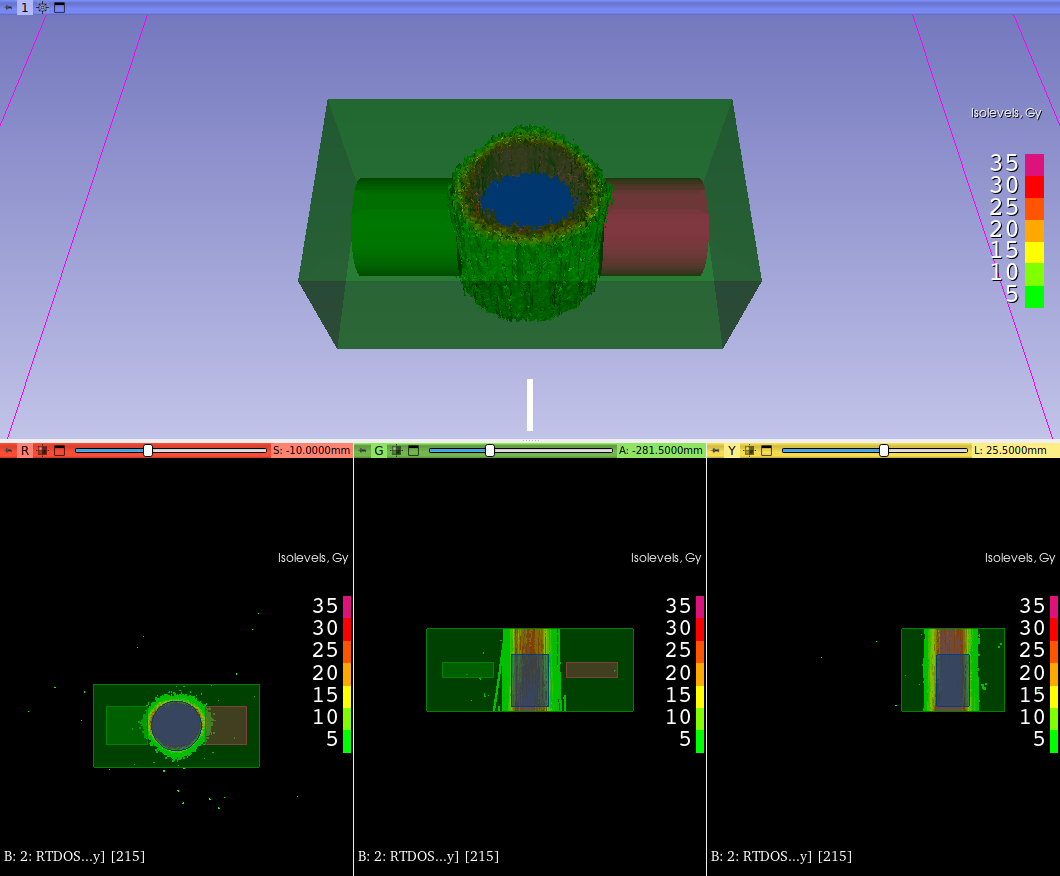
\includegraphics[width= 0.8\textwidth]{content/iso.png}
    \caption{Abgebildet sind die Isodosislinien eines CT Datensatz bei einer Bestrahlung mit einem Protonenstahl in der Pencil Beam Scanning
    Methode.}
    \label{fig:iso}
\end{figure}
Mit dem Simulationswekzeug von \enquote{TOPAS} werden so mehrer Protonen an entsprechender Stelle simuliert wobei die Teilchenanzahl in einer Größenordnung 
von insgesamt $10^8$ liegt. So werden statistische Fehler minimiert. Die deponierte Dosis kann in \enquote{Slicer3D} ausgelesen,
und anschließend durch DICOM manipulation durch den Tag $(3004, 000E)$ auf die gewünschten $60 Gy$ skaliert werden. 
Durch Hinzufügen des Tags (3004, 0002) wird wahlweise noch die Information \enquote{Gy} beigegeben.

\subsection{Aufgabe 2 b)}
Der Abbildung \ref{fig:slicer} ist eine mittlere Dosis von $60 Gy$ zu entnehmen. Die Grafik \ref{fig:dvh} verdeutlich zudem die 
Unterschreitung der Richtlinie von einer maximal Dosis $50 Gy$ und $D_{10\%} < 15 Gy$. 
\begin{figure}
    \centering
    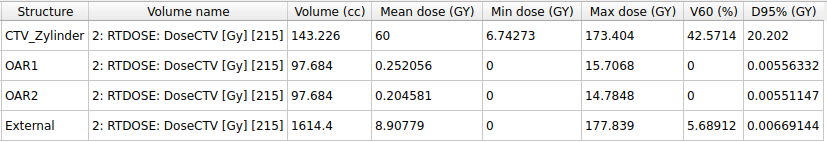
\includegraphics[width  = 0.8\textwidth]{content/slicer.png}
    \caption{Abgebildet sind ausgelesne Dosisinformationen von der Anwendung \enquote{Slicer3D} über die Bestrahlung eines CT Datensatzes.}
    \label{fig:slicer}
\end{figure}
\noindent
Von diesen Richtlinien jedoch abgesehen würde sich die Behandlung bei einem Patienten nicht durchsetzten können. 
Die maximale Dosis, abgelesen in \ref{fig:slicer} würde zu einer direkten Nekrose führen und der Heilungsprozess wäre maßgeblich 
eingeschrkänkt. Zu dem werden lediglich $\approx 42\%$ mit $60Gy$ abgedeckt, was in einem klinischen Standart über $95\%$ liegen sollte.
Alternativ kann in der Planung mit etwaigen Filtern gearbeitet, oder eine Vielfelderplaung etabliert werden
\newpage